\documentclass[preprint, 10pt]{elsarticle}

\newcommand{\mcaption}[2]{\caption{\small \em #1}\label{#2}}
\newcommand{\secref}[1]{\ref{#1}}

%\usepackage{algorithmic}
%\usepackage{algorithm}
\usepackage{amsfonts}
\usepackage[fleqn,reqno]{amsmath}
\usepackage{amssymb}
%\usepackage{amsthm}
\usepackage[titletoc]{appendix}
\usepackage{array}
%\usepackage{bm}
%\usepackage{caption}
%\usepackage[usenames]{color}
\usepackage{enumitem}
%\usepackage{epsfig}
%\usepackage{fancybox}
\usepackage{filecontents}
\usepackage[top=1.2in,bottom=1.2in,left=1in, right=1in]{geometry}
\usepackage{graphics}
%%\usepackage{ifthen}
\usepackage{lineno}
%\usepackage{mathrsfs}
%\usepackage{mdframed}
%\usepackage{multirow}
%\usepackage{palatino}
%\usepackage{showkeys} %To see the labels for now.  Will remove later
%\usepackage{stmaryrd}
%\usepackage{subfigure}
%\usepackage{paralist}
\usepackage{pgfplots}
%\usepackage{tabularx}
\usepackage{tikz}
\usepackage{todonotes}
\usetikzlibrary{arrows}
\usepackage{comment}

%%%%%%  pdftex  %%%%%%%%%%%%%%%%%%%%%%%%%%%%%%%%%%%%%%%%%%%%%%%%%%%%%%
\usepackage[pagebackref=false,bookmarks=false]{hyperref} 

\hypersetup{
  bookmarksnumbered=true,
  bookmarksopen=false,
  hypertexnames=false,      
  breaklinks=true,          
  unicode=false,
  pdffitwindow=true,        
  pdfnewwindow=true,        
  colorlinks=true,         
  linkcolor=dblue,
  anchorcolor=red,
  citecolor=dorange,
  filecolor=magenta,
  urlcolor=dblue,
  pdfstartview = FitH,
  pdfkeywords = {},
  pdfcreator = {LaTeX with hyperref package}
}



\newcommand{\bd}{{\partial}}
\newcommand{\bigO}{{\mathcal{O}}}
\newcommand{\cc}{{\mathbf{c}}}
\newcommand{\DD}{{\mathcal{D}}}
\newcommand{\eeta}{{\boldsymbol\eta}}
\newcommand{\ff}{{\mathbf{f}}}
\newcommand{\grad}{{\nabla}}
\newcommand{\II}{{\mathbf{I}}}
\newcommand{\iin}{\mathrm{in}}
\newcommand{\llambda}{{\boldsymbol\lambda}}
\newcommand{\nn}{{\mathbf{n}}}
\newcommand{\NN}{{\mathcal{N}}}
\newcommand{\out}{\mathrm{out}}
\newcommand{\rr}{{\mathbf{r}}}
\newcommand{\RR}{{\mathbb{R}}}
\renewcommand{\ss}{{\mathbf{s}}}
\newcommand{\ssigma}{{\boldsymbol\sigma}}
\newcommand{\tar}{\mathrm{tar}}
\newcommand{\uu}{{\mathbf{u}}}
\newcommand{\UU}{{\mathbf{U}}}
\newcommand{\vv}{{\mathbf{v}}}
\newcommand{\xx}{{\mathbf{x}}}
\newcommand{\xxi}{{\boldsymbol{\xi}}}
\newcommand{\yy}{{\mathbf{y}}}

\def\gap{\hspace*{.2in}}

% Derivatives
\newcommand{\pderiv}[2]{\frac{\partial #1}{\partial #2}}
\newcommand{\tderiv}[2]{\frac{d #1}{d #2}}
\newcommand{\ppd}[2]{\frac{\partial^2 #1}{{\partial #2}^2}}

% Nick's commands
\newcommand{\vsp}[1]{\vspace{#1 pc} \noindent}
\newcommand{\abs}[1]{\lvert #1 \rvert}
\newcommand{\mean}[1]{\left< #1 \right>}
\newcommand{\thL}{$\theta$--$L$}
\newcommand{\eps}{\varepsilon}
\newcommand{\Vn}{V_n}
\newcommand{\Vs}{V_s}
\newcommand{\atau}{\abs{\tau}}
\newcommand{\thalpha}{\pderiv{\theta}{\alpha}}
\newcommand{\elfun}{\zeta}
\newcommand{\thhat}{\hat{\theta}}
\newcommand{\Dt}{\Delta t}
\newcommand{\NLterm}{\mathcal{N}}
\newcommand{\Mterm}{\mathcal{M}}
\newcommand{\FourierSum}{ \sum_{k = -N_\iin /2}^{N_\iin /2-1} }
\newcommand{\atausig}{\atau^{(\sigma)}}
\newcommand{\Vnsig}{\Vn^{(\sigma)}}
\newcommand{\Vssig}{\Vs^{(\sigma)}}


\newcommand{\tauD}[1]{\tau_{#1\text{D}}}
\newcommand{\atauD}[1]{\abs{\tau_{#1\text{D}}}}

\begin{document}

\title{Methods paper for erosion}

\author[Bryan]{Bryan D.~Quaife}
\author[Nick]{M.~Nicholas J.~Moore}
\address[Nick]{Department of Mathematics and Geophysical Fluid Dynamics Institute, Florida State University, Tallahassee, FL, 32306.}
\address[Bryan]{Department of Scientific Computing and Geophysical Fluid Dynamics Institute, Florida State University, Tallahassee, FL, 32306.}

\begin{abstract} 
We consider two dimensional eroding bodies in Stokes flow
\end{abstract}

\begin{keyword}
  Stokes flow \sep Erosion \sep Boundary integral method \sep
  Fluid-structure interaction \sep Fast multipole methods 
\end{keyword}

\maketitle

%%%%%%%%%%%%%%%%%%%%%%%%%%%%%%%%%%%%%%%%%%%%%%%%%%%%%%%%%%%%%%%%%%%%%%%
\section{Introduction\label{s:intro}}

This is a methods paper
\begin{itemize}
  \item Boundary integral equation formulation
  \item How we compute the shear stress and pressure
  \item Multiple bodies
  \item Avoiding stokes paradox
  \item {\thL} formulation
  \item Regularization
\end{itemize}




%%%%%%%%%%%%%%%%%%%%%%%%%%%%%%%%%%%%%%%%%%%%%%%%%%%%%%%%%%%%%%%%%%%%%%%
\section{Formulation\label{s:formulation}} 
Let us first define the main variables used to model erosion.  We only
consider flows that are confined by a solid wall $\Gamma$ that encloses
$M$ eroding bodies.  The bodies are denoted as $\gamma_\ell$,
$\ell=1,\ldots,M$, and we write $\gamma = \gamma_1 \cup \cdots \cup
\gamma_M$.  Neglecting inertial forces, the dynamics of the fluid is
fully characterized by the position of the bodies $\xx_\ell(s,t) \in
\gamma_\ell$, where $s$ is the arclength and $t$ is time.  Given
$\xx_\ell(s,t)$, $\ell=1,\ldots,M$, derived variables include the fluid
velocity $\uu$, the pressure $p$, and the shear stress $\tau$.   On the
bounding wall, we prescribed a velocity $\UU(\xx,t)$.  Then, the
governing equations are
\begin{equation}
\label{eqn:erosionModel}
\begin{split}
  \mu \Delta \uu = \grad p, &\hspace{20pt} \xx \in \Omega, \gap &&\mbox{conservation
of momentum}\\
\grad \cdot \uu = 0, &\hspace{20pt} \xx \in \Omega, \gap
&&\mbox{conservation of mass} \\
\uu = 0, &\hspace{20pt} \xx \in \gamma, \gap &&\mbox{no slip on the
bodies} \\
\uu = \UU, &\hspace{20pt} \xx \in \Gamma, \gap &&\mbox{outer wall
velocity} \\
\dot{\xx}(t) = \abs{\tau} \nn, &\hspace{20pt} \xx \in \gamma,
&&\mbox{erosion model},
\end{split}
\end{equation}
where $\nn$ is the outward unit normal vector which points away from the
fluid, and $\mu$ is the fluid viscosity.  The outer wall is formed by
rounding off the corners of $[-3,3] \times [-1,1]$, and we enforce the
Hagen-Poiseuille flow
\begin{align*}
  \uu(\xx) = (1-y^2,0)
\end{align*}
on $\Gamma$.  The boundary of the fluid domain is $\bd\Omega = \gamma_1
\cup \cdots \cup \gamma_M \cup \Gamma$.  To minimize the boundary
effects of the inflow and outflow, we only place bodies in the center
third, $[-1,1] \times [-1,1]$, of the fluid domain.
\begin{figure}[htpb]
  \centering
  \begin{tikzpicture}[scale=1.5] 

\begin{axis}[ 
axis equal image, 
scale only axis, 
xmin=-3.04, 
xmax=3.6, 
ymin=-1.1, 
ymax=1.1, 
hide axis, 
] 

\addplot [color=black,dashed,line width=1] coordinates{ 
  (-1,-1)
  (-1,+1)
}; 

\addplot [color=black,dashed,line width=1] coordinates{ 
  (1,-1)
  (1,+1)
}; 

\addplot [color=black,solid,line width=2] coordinates{ 
(3.0000e+00,0.0000e+00)
(3.0000e+00,2.4549e-02)
(3.0000e+00,4.9127e-02)
(3.0000e+00,7.3764e-02)
(3.0000e+00,9.8491e-02)
(3.0000e+00,1.2334e-01)
(3.0000e+00,1.4834e-01)
(3.0000e+00,1.7352e-01)
(3.0000e+00,1.9891e-01)
(3.0000e+00,2.2456e-01)
(3.0000e+00,2.5049e-01)
(3.0000e+00,2.7674e-01)
(3.0000e+00,3.0334e-01)
(2.9999e+00,3.3035e-01)
(2.9999e+00,3.5779e-01)
(2.9998e+00,3.8572e-01)
(2.9997e+00,4.1417e-01)
(2.9994e+00,4.4319e-01)
(2.9991e+00,4.7282e-01)
(2.9985e+00,5.0310e-01)
(2.9975e+00,5.3407e-01)
(2.9960e+00,5.6575e-01)
(2.9938e+00,5.9814e-01)
(2.9904e+00,6.3123e-01)
(2.9854e+00,6.6493e-01)
(2.9780e+00,6.9912e-01)
(2.9673e+00,7.3358e-01)
(2.9520e+00,7.6793e-01)
(2.9306e+00,8.0171e-01)
(2.9014e+00,8.3425e-01)
(2.8625e+00,8.6481e-01)
(2.8126e+00,8.9262e-01)
(2.7510e+00,9.1700e-01)
(2.6779e+00,9.3755e-01)
(2.5944e+00,9.5418e-01)
(2.5028e+00,9.6713e-01)
(2.4051e+00,9.7688e-01)
(2.3038e+00,9.8402e-01)
(2.2007e+00,9.8911e-01)
(2.0974e+00,9.9268e-01)
(1.9948e+00,9.9514e-01)
(1.8937e+00,9.9681e-01)
(1.7944e+00,9.9794e-01)
(1.6972e+00,9.9868e-01)
(1.6022e+00,9.9917e-01)
(1.5093e+00,9.9949e-01)
(1.4185e+00,9.9969e-01)
(1.3296e+00,9.9981e-01)
(1.2425e+00,9.9989e-01)
(1.1572e+00,9.9994e-01)
(1.0734e+00,9.9997e-01)
(9.9105e-01,9.9998e-01)
(9.1003e-01,9.9999e-01)
(8.3021e-01,1.0000e+00)
(7.5146e-01,1.0000e+00)
(6.7367e-01,1.0000e+00)
(5.9674e-01,1.0000e+00)
(5.2055e-01,1.0000e+00)
(4.4501e-01,1.0000e+00)
(3.7001e-01,1.0000e+00)
(2.9547e-01,1.0000e+00)
(2.2129e-01,1.0000e+00)
(1.4738e-01,1.0000e+00)
(7.3646e-02,1.0000e+00)
(1.8370e-16,1.0000e+00)
(-7.3646e-02,1.0000e+00)
(-1.4738e-01,1.0000e+00)
(-2.2129e-01,1.0000e+00)
(-2.9547e-01,1.0000e+00)
(-3.7001e-01,1.0000e+00)
(-4.4501e-01,1.0000e+00)
(-5.2055e-01,1.0000e+00)
(-5.9674e-01,1.0000e+00)
(-6.7367e-01,1.0000e+00)
(-7.5146e-01,1.0000e+00)
(-8.3021e-01,1.0000e+00)
(-9.1003e-01,9.9999e-01)
(-9.9105e-01,9.9998e-01)
(-1.0734e+00,9.9997e-01)
(-1.1572e+00,9.9994e-01)
(-1.2425e+00,9.9989e-01)
(-1.3296e+00,9.9981e-01)
(-1.4185e+00,9.9969e-01)
(-1.5093e+00,9.9949e-01)
(-1.6022e+00,9.9917e-01)
(-1.6972e+00,9.9868e-01)
(-1.7944e+00,9.9794e-01)
(-1.8937e+00,9.9681e-01)
(-1.9948e+00,9.9514e-01)
(-2.0974e+00,9.9268e-01)
(-2.2007e+00,9.8911e-01)
(-2.3038e+00,9.8402e-01)
(-2.4051e+00,9.7688e-01)
(-2.5028e+00,9.6713e-01)
(-2.5944e+00,9.5418e-01)
(-2.6779e+00,9.3755e-01)
(-2.7510e+00,9.1700e-01)
(-2.8126e+00,8.9262e-01)
(-2.8625e+00,8.6481e-01)
(-2.9014e+00,8.3425e-01)
(-2.9306e+00,8.0171e-01)
(-2.9520e+00,7.6793e-01)
(-2.9673e+00,7.3358e-01)
(-2.9780e+00,6.9912e-01)
(-2.9854e+00,6.6493e-01)
(-2.9904e+00,6.3123e-01)
(-2.9938e+00,5.9814e-01)
(-2.9960e+00,5.6575e-01)
(-2.9975e+00,5.3407e-01)
(-2.9985e+00,5.0310e-01)
(-2.9991e+00,4.7282e-01)
(-2.9994e+00,4.4319e-01)
(-2.9997e+00,4.1417e-01)
(-2.9998e+00,3.8572e-01)
(-2.9999e+00,3.5779e-01)
(-2.9999e+00,3.3035e-01)
(-3.0000e+00,3.0334e-01)
(-3.0000e+00,2.7674e-01)
(-3.0000e+00,2.5049e-01)
(-3.0000e+00,2.2456e-01)
(-3.0000e+00,1.9891e-01)
(-3.0000e+00,1.7352e-01)
(-3.0000e+00,1.4834e-01)
(-3.0000e+00,1.2334e-01)
(-3.0000e+00,9.8491e-02)
(-3.0000e+00,7.3764e-02)
(-3.0000e+00,4.9127e-02)
(-3.0000e+00,2.4549e-02)
(-3.0000e+00,1.2246e-16)
(-3.0000e+00,-2.4549e-02)
(-3.0000e+00,-4.9127e-02)
(-3.0000e+00,-7.3764e-02)
(-3.0000e+00,-9.8491e-02)
(-3.0000e+00,-1.2334e-01)
(-3.0000e+00,-1.4834e-01)
(-3.0000e+00,-1.7352e-01)
(-3.0000e+00,-1.9891e-01)
(-3.0000e+00,-2.2456e-01)
(-3.0000e+00,-2.5049e-01)
(-3.0000e+00,-2.7674e-01)
(-3.0000e+00,-3.0334e-01)
(-2.9999e+00,-3.3035e-01)
(-2.9999e+00,-3.5779e-01)
(-2.9998e+00,-3.8572e-01)
(-2.9997e+00,-4.1417e-01)
(-2.9994e+00,-4.4319e-01)
(-2.9991e+00,-4.7282e-01)
(-2.9985e+00,-5.0310e-01)
(-2.9975e+00,-5.3407e-01)
(-2.9960e+00,-5.6575e-01)
(-2.9938e+00,-5.9814e-01)
(-2.9904e+00,-6.3123e-01)
(-2.9854e+00,-6.6493e-01)
(-2.9780e+00,-6.9912e-01)
(-2.9673e+00,-7.3358e-01)
(-2.9520e+00,-7.6793e-01)
(-2.9306e+00,-8.0171e-01)
(-2.9014e+00,-8.3425e-01)
(-2.8625e+00,-8.6481e-01)
(-2.8126e+00,-8.9262e-01)
(-2.7510e+00,-9.1700e-01)
(-2.6779e+00,-9.3755e-01)
(-2.5944e+00,-9.5418e-01)
(-2.5028e+00,-9.6713e-01)
(-2.4051e+00,-9.7688e-01)
(-2.3038e+00,-9.8402e-01)
(-2.2007e+00,-9.8911e-01)
(-2.0974e+00,-9.9268e-01)
(-1.9948e+00,-9.9514e-01)
(-1.8937e+00,-9.9681e-01)
(-1.7944e+00,-9.9794e-01)
(-1.6972e+00,-9.9868e-01)
(-1.6022e+00,-9.9917e-01)
(-1.5093e+00,-9.9949e-01)
(-1.4185e+00,-9.9969e-01)
(-1.3296e+00,-9.9981e-01)
(-1.2425e+00,-9.9989e-01)
(-1.1572e+00,-9.9994e-01)
(-1.0734e+00,-9.9997e-01)
(-9.9105e-01,-9.9998e-01)
(-9.1003e-01,-9.9999e-01)
(-8.3021e-01,-1.0000e+00)
(-7.5146e-01,-1.0000e+00)
(-6.7367e-01,-1.0000e+00)
(-5.9674e-01,-1.0000e+00)
(-5.2055e-01,-1.0000e+00)
(-4.4501e-01,-1.0000e+00)
(-3.7001e-01,-1.0000e+00)
(-2.9547e-01,-1.0000e+00)
(-2.2129e-01,-1.0000e+00)
(-1.4738e-01,-1.0000e+00)
(-7.3646e-02,-1.0000e+00)
(-5.5109e-16,-1.0000e+00)
(7.3646e-02,-1.0000e+00)
(1.4738e-01,-1.0000e+00)
(2.2129e-01,-1.0000e+00)
(2.9547e-01,-1.0000e+00)
(3.7001e-01,-1.0000e+00)
(4.4501e-01,-1.0000e+00)
(5.2055e-01,-1.0000e+00)
(5.9674e-01,-1.0000e+00)
(6.7367e-01,-1.0000e+00)
(7.5146e-01,-1.0000e+00)
(8.3021e-01,-1.0000e+00)
(9.1003e-01,-9.9999e-01)
(9.9105e-01,-9.9998e-01)
(1.0734e+00,-9.9997e-01)
(1.1572e+00,-9.9994e-01)
(1.2425e+00,-9.9989e-01)
(1.3296e+00,-9.9981e-01)
(1.4185e+00,-9.9969e-01)
(1.5093e+00,-9.9949e-01)
(1.6022e+00,-9.9917e-01)
(1.6972e+00,-9.9868e-01)
(1.7944e+00,-9.9794e-01)
(1.8937e+00,-9.9681e-01)
(1.9948e+00,-9.9514e-01)
(2.0974e+00,-9.9268e-01)
(2.2007e+00,-9.8911e-01)
(2.3038e+00,-9.8402e-01)
(2.4051e+00,-9.7688e-01)
(2.5028e+00,-9.6713e-01)
(2.5944e+00,-9.5418e-01)
(2.6779e+00,-9.3755e-01)
(2.7510e+00,-9.1700e-01)
(2.8126e+00,-8.9262e-01)
(2.8625e+00,-8.6481e-01)
(2.9014e+00,-8.3425e-01)
(2.9306e+00,-8.0171e-01)
(2.9520e+00,-7.6793e-01)
(2.9673e+00,-7.3358e-01)
(2.9780e+00,-6.9912e-01)
(2.9854e+00,-6.6493e-01)
(2.9904e+00,-6.3123e-01)
(2.9938e+00,-5.9814e-01)
(2.9960e+00,-5.6575e-01)
(2.9975e+00,-5.3407e-01)
(2.9985e+00,-5.0310e-01)
(2.9991e+00,-4.7282e-01)
(2.9994e+00,-4.4319e-01)
(2.9997e+00,-4.1417e-01)
(2.9998e+00,-3.8572e-01)
(2.9999e+00,-3.5779e-01)
(2.9999e+00,-3.3035e-01)
(3.0000e+00,-3.0334e-01)
(3.0000e+00,-2.7674e-01)
(3.0000e+00,-2.5049e-01)
(3.0000e+00,-2.2456e-01)
(3.0000e+00,-1.9891e-01)
(3.0000e+00,-1.7352e-01)
(3.0000e+00,-1.4834e-01)
(3.0000e+00,-1.2334e-01)
(3.0000e+00,-9.8491e-02)
(3.0000e+00,-7.3764e-02)
(3.0000e+00,-4.9127e-02)
(3.0000e+00,-2.4549e-02)
(3.0000e+00,0.0000e+00)
}; 

\addplot [color=black,solid,fill] coordinates{ 
(5.0000e-01,0.0000e+00)
(4.9759e-01,4.9009e-02)
(4.9039e-01,9.7545e-02)
(4.7847e-01,1.4514e-01)
(4.6194e-01,1.9134e-01)
(4.4096e-01,2.3570e-01)
(4.1573e-01,2.7779e-01)
(3.8651e-01,3.1720e-01)
(3.5355e-01,3.5355e-01)
(3.1720e-01,3.8651e-01)
(2.7779e-01,4.1573e-01)
(2.3570e-01,4.4096e-01)
(1.9134e-01,4.6194e-01)
(1.4514e-01,4.7847e-01)
(9.7545e-02,4.9039e-01)
(4.9009e-02,4.9759e-01)
(3.0616e-17,5.0000e-01)
(-4.9009e-02,4.9759e-01)
(-9.7545e-02,4.9039e-01)
(-1.4514e-01,4.7847e-01)
(-1.9134e-01,4.6194e-01)
(-2.3570e-01,4.4096e-01)
(-2.7779e-01,4.1573e-01)
(-3.1720e-01,3.8651e-01)
(-3.5355e-01,3.5355e-01)
(-3.8651e-01,3.1720e-01)
(-4.1573e-01,2.7779e-01)
(-4.4096e-01,2.3570e-01)
(-4.6194e-01,1.9134e-01)
(-4.7847e-01,1.4514e-01)
(-4.9039e-01,9.7545e-02)
(-4.9759e-01,4.9009e-02)
(-5.0000e-01,6.1232e-17)
(-4.9759e-01,-4.9009e-02)
(-4.9039e-01,-9.7545e-02)
(-4.7847e-01,-1.4514e-01)
(-4.6194e-01,-1.9134e-01)
(-4.4096e-01,-2.3570e-01)
(-4.1573e-01,-2.7779e-01)
(-3.8651e-01,-3.1720e-01)
(-3.5355e-01,-3.5355e-01)
(-3.1720e-01,-3.8651e-01)
(-2.7779e-01,-4.1573e-01)
(-2.3570e-01,-4.4096e-01)
(-1.9134e-01,-4.6194e-01)
(-1.4514e-01,-4.7847e-01)
(-9.7545e-02,-4.9039e-01)
(-4.9009e-02,-4.9759e-01)
(-9.1849e-17,-5.0000e-01)
(4.9009e-02,-4.9759e-01)
(9.7545e-02,-4.9039e-01)
(1.4514e-01,-4.7847e-01)
(1.9134e-01,-4.6194e-01)
(2.3570e-01,-4.4096e-01)
(2.7779e-01,-4.1573e-01)
(3.1720e-01,-3.8651e-01)
(3.5355e-01,-3.5355e-01)
(3.8651e-01,-3.1720e-01)
(4.1573e-01,-2.7779e-01)
(4.4096e-01,-2.3570e-01)
(4.6194e-01,-1.9134e-01)
(4.7847e-01,-1.4514e-01)
(4.9039e-01,-9.7545e-02)
(4.9759e-01,-4.9009e-02)
(5.0000e-01,-1.2246e-16)
};

\addplot [color=black,solid,fill] coordinates{ 
(8.0000e-01,5.0000e-01)
(7.9952e-01,5.0980e-01)
(7.9808e-01,5.1951e-01)
(7.9569e-01,5.2903e-01)
(7.9239e-01,5.3827e-01)
(7.8819e-01,5.4714e-01)
(7.8315e-01,5.5556e-01)
(7.7730e-01,5.6344e-01)
(7.7071e-01,5.7071e-01)
(7.6344e-01,5.7730e-01)
(7.5556e-01,5.8315e-01)
(7.4714e-01,5.8819e-01)
(7.3827e-01,5.9239e-01)
(7.2903e-01,5.9569e-01)
(7.1951e-01,5.9808e-01)
(7.0980e-01,5.9952e-01)
(7.0000e-01,6.0000e-01)
(6.9020e-01,5.9952e-01)
(6.8049e-01,5.9808e-01)
(6.7097e-01,5.9569e-01)
(6.6173e-01,5.9239e-01)
(6.5286e-01,5.8819e-01)
(6.4444e-01,5.8315e-01)
(6.3656e-01,5.7730e-01)
(6.2929e-01,5.7071e-01)
(6.2270e-01,5.6344e-01)
(6.1685e-01,5.5556e-01)
(6.1181e-01,5.4714e-01)
(6.0761e-01,5.3827e-01)
(6.0431e-01,5.2903e-01)
(6.0192e-01,5.1951e-01)
(6.0048e-01,5.0980e-01)
(6.0000e-01,5.0000e-01)
(6.0048e-01,4.9020e-01)
(6.0192e-01,4.8049e-01)
(6.0431e-01,4.7097e-01)
(6.0761e-01,4.6173e-01)
(6.1181e-01,4.5286e-01)
(6.1685e-01,4.4444e-01)
(6.2270e-01,4.3656e-01)
(6.2929e-01,4.2929e-01)
(6.3656e-01,4.2270e-01)
(6.4444e-01,4.1685e-01)
(6.5286e-01,4.1181e-01)
(6.6173e-01,4.0761e-01)
(6.7097e-01,4.0431e-01)
(6.8049e-01,4.0192e-01)
(6.9020e-01,4.0048e-01)
(7.0000e-01,4.0000e-01)
(7.0980e-01,4.0048e-01)
(7.1951e-01,4.0192e-01)
(7.2903e-01,4.0431e-01)
(7.3827e-01,4.0761e-01)
(7.4714e-01,4.1181e-01)
(7.5556e-01,4.1685e-01)
(7.6344e-01,4.2270e-01)
(7.7071e-01,4.2929e-01)
(7.7730e-01,4.3656e-01)
(7.8315e-01,4.4444e-01)
(7.8819e-01,4.5286e-01)
(7.9239e-01,4.6173e-01)
(7.9569e-01,4.7097e-01)
(7.9808e-01,4.8049e-01)
(7.9952e-01,4.9020e-01)
(8.0000e-01,5.0000e-01)
};

\addplot [color=black,solid,fill] coordinates{ 
(-6.0000e-01,6.0000e-01)
(-6.0096e-01,6.1960e-01)
(-6.0384e-01,6.3902e-01)
(-6.0861e-01,6.5806e-01)
(-6.1522e-01,6.7654e-01)
(-6.2362e-01,6.9428e-01)
(-6.3371e-01,7.1111e-01)
(-6.4540e-01,7.2688e-01)
(-6.5858e-01,7.4142e-01)
(-6.7312e-01,7.5460e-01)
(-6.8889e-01,7.6629e-01)
(-7.0572e-01,7.7638e-01)
(-7.2346e-01,7.8478e-01)
(-7.4194e-01,7.9139e-01)
(-7.6098e-01,7.9616e-01)
(-7.8040e-01,7.9904e-01)
(-8.0000e-01,8.0000e-01)
(-8.1960e-01,7.9904e-01)
(-8.3902e-01,7.9616e-01)
(-8.5806e-01,7.9139e-01)
(-8.7654e-01,7.8478e-01)
(-8.9428e-01,7.7638e-01)
(-9.1111e-01,7.6629e-01)
(-9.2688e-01,7.5460e-01)
(-9.4142e-01,7.4142e-01)
(-9.5460e-01,7.2688e-01)
(-9.6629e-01,7.1111e-01)
(-9.7638e-01,6.9428e-01)
(-9.8478e-01,6.7654e-01)
(-9.9139e-01,6.5806e-01)
(-9.9616e-01,6.3902e-01)
(-9.9904e-01,6.1960e-01)
(-1.0000e+00,6.0000e-01)
(-9.9904e-01,5.8040e-01)
(-9.9616e-01,5.6098e-01)
(-9.9139e-01,5.4194e-01)
(-9.8478e-01,5.2346e-01)
(-9.7638e-01,5.0572e-01)
(-9.6629e-01,4.8889e-01)
(-9.5460e-01,4.7312e-01)
(-9.4142e-01,4.5858e-01)
(-9.2688e-01,4.4540e-01)
(-9.1111e-01,4.3371e-01)
(-8.9428e-01,4.2362e-01)
(-8.7654e-01,4.1522e-01)
(-8.5806e-01,4.0861e-01)
(-8.3902e-01,4.0384e-01)
(-8.1960e-01,4.0096e-01)
(-8.0000e-01,4.0000e-01)
(-7.8040e-01,4.0096e-01)
(-7.6098e-01,4.0384e-01)
(-7.4194e-01,4.0861e-01)
(-7.2346e-01,4.1522e-01)
(-7.0572e-01,4.2362e-01)
(-6.8889e-01,4.3371e-01)
(-6.7312e-01,4.4540e-01)
(-6.5858e-01,4.5858e-01)
(-6.4540e-01,4.7312e-01)
(-6.3371e-01,4.8889e-01)
(-6.2362e-01,5.0572e-01)
(-6.1522e-01,5.2346e-01)
(-6.0861e-01,5.4194e-01)
(-6.0384e-01,5.6098e-01)
(-6.0096e-01,5.8040e-01)
(-6.0000e-01,6.0000e-01)
};

\addplot [color=black,solid,fill] coordinates{ 
(9.0000e-01,-6.0000e-01)
(8.9904e-01,-5.8040e-01)
(8.9616e-01,-5.6098e-01)
(8.9139e-01,-5.4194e-01)
(8.8478e-01,-5.2346e-01)
(8.7638e-01,-5.0572e-01)
(8.6629e-01,-4.8889e-01)
(8.5460e-01,-4.7312e-01)
(8.4142e-01,-4.5858e-01)
(8.2688e-01,-4.4540e-01)
(8.1111e-01,-4.3371e-01)
(7.9428e-01,-4.2362e-01)
(7.7654e-01,-4.1522e-01)
(7.5806e-01,-4.0861e-01)
(7.3902e-01,-4.0384e-01)
(7.1960e-01,-4.0096e-01)
(7.0000e-01,-4.0000e-01)
(6.8040e-01,-4.0096e-01)
(6.6098e-01,-4.0384e-01)
(6.4194e-01,-4.0861e-01)
(6.2346e-01,-4.1522e-01)
(6.0572e-01,-4.2362e-01)
(5.8889e-01,-4.3371e-01)
(5.7312e-01,-4.4540e-01)
(5.5858e-01,-4.5858e-01)
(5.4540e-01,-4.7312e-01)
(5.3371e-01,-4.8889e-01)
(5.2362e-01,-5.0572e-01)
(5.1522e-01,-5.2346e-01)
(5.0861e-01,-5.4194e-01)
(5.0384e-01,-5.6098e-01)
(5.0096e-01,-5.8040e-01)
(5.0000e-01,-6.0000e-01)
(5.0096e-01,-6.1960e-01)
(5.0384e-01,-6.3902e-01)
(5.0861e-01,-6.5806e-01)
(5.1522e-01,-6.7654e-01)
(5.2362e-01,-6.9428e-01)
(5.3371e-01,-7.1111e-01)
(5.4540e-01,-7.2688e-01)
(5.5858e-01,-7.4142e-01)
(5.7312e-01,-7.5460e-01)
(5.8889e-01,-7.6629e-01)
(6.0572e-01,-7.7638e-01)
(6.2346e-01,-7.8478e-01)
(6.4194e-01,-7.9139e-01)
(6.6098e-01,-7.9616e-01)
(6.8040e-01,-7.9904e-01)
(7.0000e-01,-8.0000e-01)
(7.1960e-01,-7.9904e-01)
(7.3902e-01,-7.9616e-01)
(7.5806e-01,-7.9139e-01)
(7.7654e-01,-7.8478e-01)
(7.9428e-01,-7.7638e-01)
(8.1111e-01,-7.6629e-01)
(8.2688e-01,-7.5460e-01)
(8.4142e-01,-7.4142e-01)
(8.5460e-01,-7.2688e-01)
(8.6629e-01,-7.1111e-01)
(8.7638e-01,-6.9428e-01)
(8.8478e-01,-6.7654e-01)
(8.9139e-01,-6.5806e-01)
(8.9616e-01,-6.3902e-01)
(8.9904e-01,-6.1960e-01)
(9.0000e-01,-6.0000e-01)
};

\addplot [color=black,solid,fill] coordinates{ 
(-6.4000e-01,-5.0000e-01)
(-6.4029e-01,-4.9412e-01)
(-6.4115e-01,-4.8829e-01)
(-6.4258e-01,-4.8258e-01)
(-6.4457e-01,-4.7704e-01)
(-6.4708e-01,-4.7172e-01)
(-6.5011e-01,-4.6667e-01)
(-6.5362e-01,-4.6194e-01)
(-6.5757e-01,-4.5757e-01)
(-6.6194e-01,-4.5362e-01)
(-6.6667e-01,-4.5011e-01)
(-6.7172e-01,-4.4708e-01)
(-6.7704e-01,-4.4457e-01)
(-6.8258e-01,-4.4258e-01)
(-6.8829e-01,-4.4115e-01)
(-6.9412e-01,-4.4029e-01)
(-7.0000e-01,-4.4000e-01)
(-7.0588e-01,-4.4029e-01)
(-7.1171e-01,-4.4115e-01)
(-7.1742e-01,-4.4258e-01)
(-7.2296e-01,-4.4457e-01)
(-7.2828e-01,-4.4708e-01)
(-7.3333e-01,-4.5011e-01)
(-7.3806e-01,-4.5362e-01)
(-7.4243e-01,-4.5757e-01)
(-7.4638e-01,-4.6194e-01)
(-7.4989e-01,-4.6667e-01)
(-7.5292e-01,-4.7172e-01)
(-7.5543e-01,-4.7704e-01)
(-7.5742e-01,-4.8258e-01)
(-7.5885e-01,-4.8829e-01)
(-7.5971e-01,-4.9412e-01)
(-7.6000e-01,-5.0000e-01)
(-7.5971e-01,-5.0588e-01)
(-7.5885e-01,-5.1171e-01)
(-7.5742e-01,-5.1742e-01)
(-7.5543e-01,-5.2296e-01)
(-7.5292e-01,-5.2828e-01)
(-7.4989e-01,-5.3333e-01)
(-7.4638e-01,-5.3806e-01)
(-7.4243e-01,-5.4243e-01)
(-7.3806e-01,-5.4638e-01)
(-7.3333e-01,-5.4989e-01)
(-7.2828e-01,-5.5292e-01)
(-7.2296e-01,-5.5543e-01)
(-7.1742e-01,-5.5742e-01)
(-7.1171e-01,-5.5885e-01)
(-7.0588e-01,-5.5971e-01)
(-7.0000e-01,-5.6000e-01)
(-6.9412e-01,-5.5971e-01)
(-6.8829e-01,-5.5885e-01)
(-6.8258e-01,-5.5742e-01)
(-6.7704e-01,-5.5543e-01)
(-6.7172e-01,-5.5292e-01)
(-6.6667e-01,-5.4989e-01)
(-6.6194e-01,-5.4638e-01)
(-6.5757e-01,-5.4243e-01)
(-6.5362e-01,-5.3806e-01)
(-6.5011e-01,-5.3333e-01)
(-6.4708e-01,-5.2828e-01)
(-6.4457e-01,-5.2296e-01)
(-6.4258e-01,-5.1742e-01)
(-6.4115e-01,-5.1171e-01)
(-6.4029e-01,-5.0588e-01)
(-6.4000e-01,-5.0000e-01)
};

%\draw[step=50] (0,0) grid (1200,300);

\node[font = \Huge,color=black] at (500,110) {$\Omega$};
\node[font = \normalsize,color=red] at (338,122) {$\nn$};
\node[font = \normalsize,color=red] at (342,158) {$\ss$};
\path[->,line width=1.2](240,90) edge (260,100);
\node at (225,90) {$\gamma_k$};
\path[->,line width=1.2,color=black](140,50) edge (120,14);
\node[font = \Large,color=black] at (150,70) {$\Gamma$};

\foreach \y in {-0.7,-0.5,...,0.7}
\addplot[color=black,line width = 1.0pt,solid,->]
plot coordinates{
  (-3,\y)
  (-3+0.6*(1-\y*\y),\y)
};

\foreach \y in {-0.7,-0.5,...,0.7}
\addplot[color=black,line width = 1.0pt,solid,->]
plot coordinates{
  (3,\y)
  (3+0.6*(1-\y*\y),\y)
};

\addplot[color=red,line width=0.5pt,solid,->]
plot coordinates{
  (0.3865,0.3172)
  (0.0966,0.0793)
};

\addplot[color=red,line width=0.5pt,solid,->]
plot coordinates{
  (0.3865,0.3172)
  (0.1486,0.6071)
};


\end{axis}

\end{tikzpicture}


  \caption{\label{fig:schematic} A schematic for the governing
    equations.  A no-slip boundary condition is imposed on each body
    $\gamma_\ell$ whose unit normal points outward relative to the
    geometry.  On the outer geometry $\Gamma$, a pipe flow is imposed.
    The bodies are eroded at a rate that is proportional to the
    magnitude of the shear stress applied by the Stokesian fluid.  The
    bodies are constrained to the middle third of the channel that is
    located between the dashed lines.}
\end{figure}

We use a quasi-static approximation.  That is, at each time step, we
freeze the geometry, solve the incompressible Stokes equations, and then
update the geometry according to the erosion model.  A flow diagram is
illustrated in Figure~\ref{fig:workflow}.  The two steps inside the red
rectangle describes a time step in the quasi-static approximation
\begin{figure}[htpb]
  \centering
  \tikzstyle{block} = [rectangle, draw, fill=blue!20, text width=11em, text centered, rounded corners, minimum height=4em]
\tikzstyle{line} = [draw, -latex', line width=2pt]

\begin{tikzpicture}[node distance = 2cm, auto]
% Place nodes
\node[block] (init) {{\bf INITIALIZE MODEL} \\ 
\begin{itemize}[noitemsep,topsep=0pt,parsep=0pt,partopsep=0pt]
  \item initialize bodies 
  \item select $N$, $\Delta t$, $\epsilon$
\end{itemize}
};


\node[block, below of=init, node distance=10em] (stokes) {{\bf FLUID
SOLVER} \\
\begin{itemize}[noitemsep,topsep=0pt,parsep=0pt,partopsep=0pt]
  \item solve incompressible Stokes equations 
  \item compute shear stress
\end{itemize}
};


\node[block, right of=stokes, node distance=14em] (thetaL) {{\bf ERODE
BODIES} \\
\begin{itemize}[noitemsep,topsep=0pt,parsep=0pt,partopsep=0pt]
  \item Compute and smooth normal velocity
  \item Update $\theta$ and $L$
  \item Compute new pore shapes
\end{itemize}
};


\node[block, right of=init, node distance=14em] (QOI) {{\bf COMPUTE
QUANTITIES OF INTEREST} \\
\begin{itemize}[noitemsep,topsep=0pt,parsep=0pt,partopsep=0pt]
  \item pressure
  \item drag
  \item velocity
\end{itemize}
};

\node[block, right of=QOI, node distance=14em,yshift=-5em] (output)
{{\bf WRITE TO FILE} \\
\begin{itemize}[noitemsep,topsep=0pt,parsep=0pt,partopsep=0pt]
  \item Geometry
  \item Density function
  \item Pressure
  \item Drag
\end{itemize}
};


%% draw rounded rectangle around the time stepping routines
\draw[rounded corners=15pt,red,line width=2pt]
  (-2.5,-5.2) rectangle ++(9.8,3.4);

  
%% Draw edges
\path [line] (init) -- (stokes);
\path [line] ([yshift=1em]stokes.east) -- ([yshift=1em]thetaL.west);
\path [line] ([yshift=-1em]thetaL.west) -- ([yshift=-1em]stokes.east);
\path [line] (stokes) -- (QOI.west);
\path [line] (QOI.east) -- ([yshift = 2em]output.west);
\path [line] (thetaL.east) -- ([yshift = -2em]output.west);


\end{tikzpicture}

  \caption{\label{fig:workflow}A caption.}
\end{figure}

Our erosion model is based on the shear stress, and this model is
discussed in more detail in Section~\ref{sec:erosion}.  We then describe
how the incompressible Stokes equations are solved in $\Omega$ using a
boundary integral equation in Section~\ref{sec:bies}.  Then, in
Section~\ref{sec:qois}, we discuss how the shear stress, pressure, and
drag can all be readily computed.  


%%%%%%%%%%%%%%%%%%%%%%%%%%%%%%%%%%%%%%%%%%%%%%%%%%%%%%%%%%%%%%%%%%%%%%%
\subsection{Erosion Model} 
\label{sec:erosion}

To model erosion, we the normal velocity is prescribed to be
proportional to the absolute value of the shear stress.  The constant of
proportionality sets the time scale, and we set its value to be 1
\begin{align}
  \dot{\xx}(t) = \abs{\tau} \nn.
  \label{eqn:bodyEvolution}
\end{align}

\todo[inline]{Describe the erosion model and its justification}
\cite{moo-ris-chi-zha-she2013}


%%%%%%%%%%%%%%%%%%%%%%%%%%%%%%%%%%%%%%%%%%%%%%%%%%%%%%%%%%%%%%%%%%%%%%%
\subsection{Boundary Integral Equation Formulation} 
\label{sec:bies}
Here we describe a boundary integral equation for the governing
equations.   This requires solving the incompressible Stokes equations
with Dirichlet boundary conditions 
\begin{alignat*}{3}
  \mu\Delta \uu &= \grad p, \qquad && \xx \in \Omega, \\
  \grad \cdot \uu &= 0,   && \xx \in \Omega, \\
  \uu &= \ff,  && \xx \in \bd\Omega,
\end{alignat*}
and also computing several quantities of interest, including the shear
stress.  The viscosity $\mu$ sets the time scale, and we will assume
that $\mu=1$.  We start by defining the double-layer potential, which is
the convolution of the stresslet with a density function
$\eeta:\bd\Omega \rightarrow \RR^2$,
\begin{align}
  \DD[\eeta](\xx) = \frac{1}{\pi} \int_{\bd\Omega} 
    \frac{\rr \cdot \nn}{\rho^2} \frac{\rr \otimes \rr}{\rho^2} 
    \eeta(\yy) \, ds_\yy, \quad \xx \in \Omega,
    \label{eqn:velocityDLP}
\end{align}
where $\rr = \xx - \yy$, $\rho = \|\rr\|$, and $\nn$ is the unit outward
normal at $\yy$.  For any density function $\eeta$, the double-layer
potential satisfies the incompressible Stokes equations, but it can not
capture velocity fields corresponding to rigid body
motions~\cite{pow-mir1987}.  A standard method to remove this rank
deficiency is to complement the double-layer potential with a Stokeslets
and rotlets centered inside each interior body
\begin{align}
  S[\llambda_\ell,\cc_\ell] = \frac{1}{4\pi} \left(-\log \rho \II + 
    \frac{\rr \otimes \rr}{\rho^2} \right)\llambda_\ell
  \quad \text{and} \quad
  R[\xi_\ell,\cc_\ell] = \frac{\rr^\perp}{\rho^2}\xi_\ell, 
  \quad \ell=1,\ldots,M,
  \label{eqn:stokeslet_rotlet}
\end{align}
where  $\rr = \xx - \cc_\ell$, $\cc_\ell$ is a point inside the
$\ell^{th}$ body, $\rr^\perp = (r_2,-r_1)$, and $\rho = \|\rr\|$.  Then,
any solution of the Stokes equations with a Dirichlet boundary condition
$\ff$ can be written in terms of the completed double-layer potential
\begin{align}
  \label{eqn:completed_DLP}
  \uu(\xx) = \DD[\eeta](\xx) + 
    \sum_{\ell=1}^{M} S[\llambda_\ell,\cc_\ell](\xx) +
    \sum_{\ell=1}^{M} R[\xi_\ell,\cc_\ell](\xx), \quad \xx \in \Omega,
\end{align}
where the density function, Stokeslets, and rotlets satisfy
\begin{subequations}
\label{eqn:completed_BIE}
\begin{align}
  \ff(\xx) &= -\frac{1}{2}\eeta(\xx) + \DD[\eeta](\xx) + 
      \sum_{\ell=1}^{M} S[\llambda_\ell,\cc_\ell](\xx) +
      \sum_{\ell=1}^{M} R[\xi_\ell,\cc_\ell](\xx) + \NN_0[\eeta](\xx),
      \quad \xx \in \bd\Omega, 
      \label{eqn:DLP}\\
  \llambda_\ell &= \frac{1}{2\pi}\int_{\gamma_\ell} \eeta(\yy) \, ds_\yy,
  \quad \ell=1,\ldots,M,
  \label{eqn:stokeslet} \\
  \xi_\ell &= \frac{1}{2\pi}\int_{\gamma_\ell} \yy^\perp \cdot \eeta(\yy)
  \, ds_\yy, \quad \ell=1,\ldots,M.
  \label{eqn:rotlet}
\end{align}
\end{subequations}
Here,
\begin{align*}
  \NN_0[\eeta](\xx) = \int_{\Gamma} 
    (\nn(\xx) \otimes \nn(\yy))\eeta(\yy) \, ds_\yy
\end{align*}
is being used to remove the rank one null space that results from the
compatibility constraint that results from the flux-free requirement of
$\ff$.


%%%%%%%%%%%%%%%%%%%%%%%%%%%%%%%%%%%%%%%%%%%%%%%%%%%%%%%%%%%%%%%%%%%%%%%
\subsection{Layer Potentials for Quantities of Interest}
\label{sec:qois}
There are several quantities besides the velocity that need to be
computed.  First, the governing equations~\eqref{eqn:erosionModel}
require the shear stress along $\gamma_\ell$.  In addition, to study
characteristics of the flow, the vorticity, pressure, and drag, and
resistivity will also be computed.  Once
equation~\eqref{eqn:completed_DLP} is solved for the density function,
Stokeslets, and rotlets, all of these quantities can be computed by
evaluating layer potentials that we now derive.

%%%%%%%%%%%%%%%%%%%%%%%%%%%%%%%%%%%%%%%%%%%%%%%%%%%%%%%%%%%%%%%%%%%%%%%
\subsubsection{Shear Stress}
The shear stress is
\begin{align*}
  \tau = -\left(\nabla \uu + \nabla \uu^T \right)\nn \cdot \ss,
\end{align*}
where $\ss$ and $\nn$ are the unit tangent and normal vectors,
respectively (Figure~\ref{fig:schematic}).  The velocity field of the
completed double-layer potential~\eqref{eqn:completed_DLP} involves
three terms: the double-layer potential $\DD$, the Stokeslets $S$, and
the rotlets $R$.  We first compute the deformation tensor $\ssigma =
\frac{1}{2}(\nabla\uu + \nabla\uu^T)$ for each of these terms
individually.

The deformation tensor of the double-layer
potential~\eqref{eqn:velocityDLP} at $\xx \in \Omega$ is
\begin{equation}
  \label{eqn:shearStressDLP}
  \begin{aligned}
  \ssigma^\DD(\xx) = \frac{1}{2\pi}\int_{\bd\Omega} &\left(
    2\frac{\rr \cdot \nn}{\rho^2} \frac{\rr \cdot \eeta}{\rho^2} \II + 
    \frac{\rr \cdot \eeta}{\rho^4} (\nn \otimes \rr + \rr \otimes \nn) 
    \right. \\
    &\left.
    +\frac{\rr \cdot \nn}{\rho^4} (\eeta \otimes \rr + \rr \otimes \eeta) - 
    8\frac{(\rr \cdot \nn)(\rr \cdot \eeta)}{\rho^6}(\rr \otimes \rr)
  \right) \eeta(\yy) ds_\yy.
  \end{aligned}
\end{equation}
We require the deformation tensor on $\bd\Omega$, and this requires
taking the limit of equation~\eqref{eqn:shearStressDLP} when $\xx$ tends
to $\xx_0 \in \bd\Omega$.  The limiting value is given
by~\cite{qua-bir2014a}
\begin{align*}
  \lim_{\substack{\xx \rightarrow \xx_0 \\ \xx \in \Omega}}\sigma_\DD(\xx) =
  J[\eeta](\xx_0) + \ssigma^\DD(\xx_0), \quad \xx_0 \in \bd\Omega,
\end{align*} 
where
\begin{align}
  J[\eeta](\xx_0) = \frac{1}{2}\left(\pderiv{\eeta}{\ss} 
    \cdot \ss\right) \left[ 
  \begin{array}{cc}
    s_x^2 - s_y^2 & 2s_x s_y \\ 2s_x s_y & s_y^2 - s_x^2
  \end{array}\right].
  \label{eqn:shearStressJump}
\end{align}
The deformation tensor of the Stokeslets and
rotlets~\eqref{eqn:stokeslet_rotlet} are
\begin{equation}
  \label{eqn:shearStressSR}
  \begin{aligned}
  \ssigma^S(\xx_0) &= \sum_{\ell=1}^{M}
    \frac{\rr \cdot \llambda_\ell}{4\pi\rho^2} \left(
    \II - \frac{2}{\rho^2} \rr \otimes \rr \right),  \\
  \ssigma^R(\xx_0) &= -\sum_{\ell=1}^M
    \frac{\xi_\ell}{\rho^4} \left(\rr \otimes \rr^\perp + 
    \rr^\perp \otimes \rr \right),
  \end{aligned}
\end{equation}
where $\rr = \xx - \cc_\ell$, $\cc_\ell$ is the point chosen inside body
$\gamma_\ell$, and $\rho = \|\rr_\ell\|$.  Now that the deformation
tensor of each component of the completed double-layer potential is
computed, the shear stress at $\xx_0 \in \bd\Omega$ is
\begin{align*}
  \tau = -2 \left(J[\eeta](\xx_0) + \ssigma^\DD(\xx_0) + 
    \ssigma^S(\xx_0) + \ssigma^R(\xx_0)\right) \nn \cdot \ss.
\end{align*}

%%%%%%%%%%%%%%%%%%%%%%%%%%%%%%%%%%%%%%%%%%%%%%%%%%%%%%%%%%%%%%%%%%%%%%%
\subsubsection{Vorticity}
For the Stokes equations, on boundaries that have a no-slip boundary
condition, the shear stress is equivalent to the vorticity $w = v_x -
u_y$.  Therefore, to compute $w(\xx)$ for $\xx \in \overline{\Omega}$,
we only need to compute $w(\xx)$ for $\xx \in \Omega$.  As we did for
the shear stress, we compute the vorticity due to the double-layer
potential, Stokeslets, and rotlets individually.  The vorticity of the
double-layer potential~\eqref{eqn:velocityDLP} at $\xx \in \Omega$ is
\begin{align}
  w^{\DD}(\xx) = -\frac{1}{\pi}\int_{\bd\Omega} 
    \frac{(\rr \cdot \nn^\perp) + (\rr \cdot \nn)}{\rho^4}
    (\rr \cdot \eeta) ds_{\yy}.
  \label{eqn:vorticityDLP}
\end{align}
The vorticity due to the Stokeslet is
\begin{align*}
  w^S(\xx) = -\frac{1}{\pi} \sum_{\ell=1}^{M} 
    \frac{\rr \cdot \llambda_\ell^\perp}{\rho^2},
\end{align*}
and the vorticity of a rotlet is zero.  Therefore, the vorticity at $\xx
\in \Omega$ is
\begin{align*}
  w(\xx) = w^\DD(\xx) + w^S(\xx).
\end{align*}


%%%%%%%%%%%%%%%%%%%%%%%%%%%%%%%%%%%%%%%%%%%%%%%%%%%%%%%%%%%%%%%%%%%%%%%
\subsubsection{Pressure}
To compute the pressure at $\xx \in \overline{\Omega}$, we follow the
same procedure used for the shear stress.  We start by computing the
pressure of the double-layer potential for $\xx \in \Omega$ and add the
appropriate jump if $\xx \in \Gamma$. For $\xx \in \Omega$, the pressure
is
\begin{align}
  p^{D}(\xx) = -\frac{1}{\pi}\int_{\bd\Omega} \frac{1}{\rho^2}
    \left(I - 2 \frac{\rr \otimes \rr}{\rho^2}\right) 
    \nn \cdot \eeta(\yy) \,ds_\yy.
    \label{eqn:pressureDLP}
\end{align}
To compute the pressure at $\xx_0 \in \bd\Omega$, we consider the limit
as $\xx$ tends to $\xx_0$.  The limiting value is given
by~\cite{qua-bir2014a}
\begin{align}
  \lim_{\substack{\xx \rightarrow \xx_0 \\ \xx \in \Omega}}p^\DD(\xx) =  
    \pderiv{\eeta}{\ss} \cdot \ss + p^{\DD}(\xx_0).
  \label{eqn:pressureJump}
\end{align}
The pressure due to the Stokeslets is
\begin{align}
  p^S(\xx_0) = \sum_{\ell=1}^{M}\frac{\rr \cdot \llambda_\ell}{2\pi\rho^2},
  \label{eqn:shearPressureSR}
\end{align}
and the pressure due to the rotlets is zero.  Therefore, the pressure is
\begin{align*}
  p(\xx) &= p^{\DD}(\xx) + p^{S}(\xx), \quad &&\xx \in \Omega,\\
  p(\xx) &= \pderiv{\eeta}{\ss} \cdot \ss + p^{\DD}(\xx) + 
              p^{S}(\xx), && \xx \in \bd\Omega.
\end{align*}

%%%%%%%%%%%%%%%%%%%%%%%%%%%%%%%%%%%%%%%%%%%%%%%%%%%%%%%%%%%%%%%%%%%%%%%
\subsubsection{Drag}
\todo[inline]{check all signs in this section.  Fortran code assumes a
normal pointing into the eroding body and a tangent vector that
corresponds to a couterclockwise parameterization}
With the pressure and shear stress, the drag on a single body with
boundary $\gamma_\ell$ is
\begin{align}
  F_D = \int_{\gamma_\ell} (-p \nn + \tau \ss)\,ds.
  \label{eqn:drag}
\end{align}

%%%%%%%%%%%%%%%%%%%%%%%%%%%%%%%%%%%%%%%%%%%%%%%%%%%%%%%%%%%%%%%%%%%%%%%
\subsubsection{Resistivity}
\begin{align}
  some equation
  \label{eqn:resistivity}
\end{align}



%%%%%%%%%%%%%%%%%%%%%%%%%%%%%%%%%%%%%%%%%%%%%%%%%%%%%%%%%%%%%%%%%%%%%%%
\section{Numerical Methods\label{s:method}} 
There are three main numerical methods that need to be developed:~the
boundary integral equation solver for
equation~\eqref{eqn:completed_BIE}, computing the quantities of interest
in Section~\ref{sec:qois}, and updating the shape of the eroding bodies
with equation~\eqref{eqn:bodyEvolution}.  So that we can form stable
simulations with long time horizons, we use numerical methods that
achieve spectral accuracy in space, fourth-order accuracy in time, and
maintain an equispaced discretization of the bodies.

In Section~\ref{sec:spatial_discretization}, we describe how the
geometry is represented.  Then, Sections~\ref{sec:on_boundary}
and~\ref{sec:off_boundary} describe how the velocity and other
quantities of interest are computed at points on and off the boundary,
respectively.  Section~\ref{sec:fmm} describes how the layer potentials
are computed efficiently.  Finally, in Section~\ref{sec:thetaL}, methods
used to update the shape are described.


%%%%%%%%%%%%%%%%%%%%%%%%%%%%%%%%%%%%%%%%%%%%%%%%%%%%%%%%%%%%%%%%%%%%%%%
\subsection{Spatial Discretization}
\label{sec:spatial_discretization}
Each body is represented with $N_\iin$ points as the Fourier series
\begin{align*}
  \xx^\ell(\alpha) = \sum_{k = -N_\iin /2}^{N_\iin /2-1} 
    \hat{x}_k^\ell e^{ik\alpha}, \quad \ell=1,\ldots,M.
\end{align*}
The exterior geometry is represented with a Fourier series using
$N_\out$ points.  Derivatives of the shape are computed in Fourier space
\begin{align*}
  \frac{d\xx(\alpha)}{d\alpha} = 
    \sum_{k = -N_\out /2}^{N_\out /2-1} ik\hat{x}_k e^{ik\alpha}.
\end{align*}


%%%%%%%%%%%%%%%%%%%%%%%%%%%%%%%%%%%%%%%%%%%%%%%%%%%%%%%%%%%%%%%%%%%%%%%
\subsection{Quadrature: On Boundary Calculations} 
\label{sec:on_boundary}
We start by discussing the quadrature methods that are used to compute
the velocity~\eqref{eqn:DLP}, shear stress~\eqref{eqn:shearStressDLP},
pressure~\eqref{eqn:pressureDLP}, and drag~\eqref{eqn:drag} at target
points on the boundary of the domain.  The velocity on $\bd\Omega$ is
required to solve the integral equation~\eqref{eqn:completed_BIE} for
the density function, Stokeslets and rotlets.  Once these are computed,
computing the shear stress, pressure, and drag is a post-processing
step.  All these integrals involve integrands that are periodic.  For
smooth integrands, the trapezoid rule guarantees spectral
accuracy~\cite{tre-wei2014}.  However, some of the integrands contain a
singularity whose strength will be reduced with singularity subtraction,
and then spectral accuracy is achieved with odd-even
integration~\cite{sid-isr1988} must be used.

%%%%%%%%%%%%%%%%%%%%%%%%%%%%%%%%%%%%%%%%%%%%%%%%%%%%%%%%%%%%%%%%%%%%%%%
\subsubsection{Velocity}
To numerically evaluate the completed double-layer
potential~\eqref{eqn:completed_BIE}, we le $N = MN_\iin + N_\out$ be the
total number of discretization points of $\bd\Omega$.  The double-layer
potential in~\eqref{eqn:DLP} is discretized with the trapezoid rule as
\begin{align}
  \DD[\eeta](\xx_i) = \sum_{j=1}^{N} K(\xx_i,\xx_j) \eeta(\xx_j) 
      \Delta s_{j}, \quad i=1,\ldots,N,
  \label{eqn:trapDLP}
\end{align}
where $\Delta s_j$ is the arclength term of $\bd\Omega$ at
$\xx_j$, and
\begin{align*}
  K(\xx,\yy) = \frac{1}{\pi} \frac{\rr \cdot \nn}{\rho^2} 
      \frac{\rr \otimes \rr}{\rho^2},
\end{align*}
where $\rr = \xx - \yy$ and $\rho = \|\rr\|$, is the kernel of the
double-layer potential.  The diagonal term of~\eqref{eqn:trapDLP} is
replaced with the limiting value of the double-layer potential
\begin{align*}
  D(\xx,\xx) = -\frac{\kappa(\xx)}{2\pi}(\ss(\xx) \otimes \ss(\xx)),
\end{align*}
where $\kappa(\xx)$ is the curvature and $\ss(\xx)$ is the unit tangent
vector at $\xx \in \bd\Omega$.  The strengths of the
Stokeslets~\eqref{eqn:stokeslet} and the rotlets~\eqref{eqn:rotlet} are
also discretized with the trapezoid rule.  Applying this discretization
strategy to~\eqref{eqn:completed_BIE}, the dense linear system that
needs to be solved is
\begin{equation}
  \label{eqn:completed_BIE_discretized}
  \begin{aligned}
    \ff(\xx_i) &= -\frac{1}{2}\ssigma(\xx_i) + \sum_{j=1}^{N} 
      K(\xx_i,\xx_j) \eeta(\xx_j) \Delta s_{j} + 
      \sum_{\ell=1}^M S[\llambda_\ell,\cc_\ell](\xx_i) \\
      &\hspace{40pt}
      +\sum_{\ell=1}^M R[\xi_\ell,\cc_\ell](\xx_i) 
      +\sum_{\xx_j \in \Gamma} (\nn(\xx_i) \otimes
      \nn(\xx_j))\eeta(\xx_j), \\
    \llambda_\ell &= \sum_{\xx_i \in \gamma_\ell} \eeta(\xx_i) 
      \Delta s_i, \\ 
    \mu_\ell &= \sum_{\xx_i \in \gamma_\ell}
      {(\xx_i - \cc_\ell)}^\perp \cdot \eeta(\xx_i) \Delta s_i,
  \end{aligned}
\end{equation}
for $i=1,\ldots,N$, $\ell=1,\ldots,M$.  Since all the integrands are
smooth and periodic, by using the trapezoid rule, we are guaranteed that
the numerical solutions converges to the true solution with spectral
accuracy.

%%%%%%%%%%%%%%%%%%%%%%%%%%%%%%%%%%%%%%%%%%%%%%%%%%%%%%%%%%%%%%%%%%%%%%%
\subsubsection{Shear Stress}
We have decomposed the deformation tensor into the contributions due to
three different terms.  The contributions from the Stokeslets and the
rotlets can be directly evaluated since $\rr \neq 0$ for all $\xx \in
\gamma$.  However, the kernel of the deformation tensor due to the
double-layer potential~\eqref{eqn:shearStressDLP} 
\begin{align*}
  K_\ssigma(\xx,\yy)\eeta(\yy) &= \frac{1}{2\pi} \left(
    2\frac{\rr \cdot \nn}{\rho^2} \frac{\rr \cdot \eeta}{\rho^2} \II + 
    \frac{\rr \cdot \eeta}{\rho^4} (\nn \otimes \rr + \rr \otimes \nn)
    \right. \\ & \hspace{25pt}+ \left.
    \frac{\rr \cdot \nn}{\rho^4} (\eeta \otimes \rr + \rr \otimes \eeta) - 
    8\frac{(\rr \cdot \nn)(\rr \cdot \eeta)}{\rho^6}(\rr \otimes \rr)
  \right),
\end{align*}
has a singularity that is asymptotic to $\bigO(\rho^{-2})$ when $\yy
\rightarrow \xx$.  The singularity strength can be reduced since the
velocity corresponding to a constant density function is
constant~\cite{poz1992}.  Therefore, the deformation tensor of the
double-layer potential is equivalent to
\begin{align*}
  \ssigma^{\DD}(\xx) = \int_{\bd\Omega}K_\ssigma(\xx,\yy)
      (\eeta(\yy) - \eeta(\xx)) \, ds_{\yy}, \quad \xx \in \bd\Omega.
\end{align*}
This expression for the deformation tensor has a singularity that is
asymptotic to $\bigO(\rho^{-1})$ when $\yy \rightarrow \xx$.  Finally,
to achieve spectral accuracy, we apply odd-even
integration~\cite{sid-isr1988}.  That is, the deformation tensor due to
the double-layer potential at a discretization point $\xx_i$ on body
$\gamma_\ell$, with $i$ being odd, is approximated as
\begin{align}
  \ssigma^{\DD}(\xx_i) = \sum_{\xx_j \notin \gamma_\ell}
    K_\ssigma(\xx_i,\xx_j) \eeta(\xx_j) \Delta s_j + 
  \sum_{\substack{\xx_j \in \gamma_\ell \\ j \: \mathtt{even}}}
    K_\ssigma(\xx_i,\xx_j) (\eeta(\xx_j) - \eeta(\xx_i)) \Delta s_j,
  \label{eqn:stressOddEven}
\end{align}
and a similar approximation is used when $i$ is even.  The deformation
tensor due to the Stokeslets and rotlets is given in
equation~\eqref{eqn:shearStressSR}.  Finally, the jump in the
deformation tensor~\eqref{eqn:shearStressJump} is added, and the
required arclength derivative is computed in Fourier space.  Then, the
shear stress can be computed by computing the deformation tensor in the
normal vector, and taking the inner product with the tangent vector.

%%%%%%%%%%%%%%%%%%%%%%%%%%%%%%%%%%%%%%%%%%%%%%%%%%%%%%%%%%%%%%%%%%%%%%%
\subsubsection{Pressure}
Similar to the shear stress, the singularity of the pressure
corresponding to the double-layer potential~\eqref{eqn:pressureDLP} is
too strong for the trapezoid rule to be directly applied.  Therefore, we
again subtract a constant density function and write the pressure as
\begin{align*}
  p^\DD(\xx) = -\frac{1}{\pi}\int_{\bd\Omega} \frac{1}{\rho^2}
    \left(I - 2 \frac{\rr \otimes \rr}{\rho^2}\right) 
    \nn \cdot (\eeta(\yy) - \eeta(\xx)) \,ds_\yy, 
    \quad \xx \in \bd\Omega
\end{align*}
Then, identical to how the shear stress is
computed~\eqref{eqn:stressOddEven}, odd-even integration is used to
evaluate this layer potential for pressure.  The pressure due to the
Stokeslets are given in equation~\eqref{eqn:shearPressureSR}.  Finally,
to add the jump condition~\eqref{eqn:pressureJump}, Fourier
differentiation is used to compute the arclength derivative. 


%%%%%%%%%%%%%%%%%%%%%%%%%%%%%%%%%%%%%%%%%%%%%%%%%%%%%%%%%%%%%%%%%%%%%%%
\subsubsection{Drag}



%%%%%%%%%%%%%%%%%%%%%%%%%%%%%%%%%%%%%%%%%%%%%%%%%%%%%%%%%%%%%%%%%%%%%%%
\subsection{Quadrature: Off Boundary Calculations} 
\label{sec:off_boundary}
To analyze the flow, we compute quantities at target points that are in
the interior of the domain.  In particular, we develop numerical methods
to compute the velocity~\eqref{eqn:velocityDLP},
pressure~\eqref{eqn:pressureDLP}, vorticity~\eqref{eqn:vorticityDLP} and
resistivity~\eqref{eqn:resistivity}.  Since the target points are not on
the boundary of the domain, all the integrals, except for the
resistivity, involve integrands that are both periodic and smooth.
However, when the target points are close to the boundary of the domain,
the integrand becomes nearly-singular, and these large derivatives
result in a loss of accuracy that needs to be rectified.  We will be
adopting a near-singular integration scheme that allows us to compute
all quantities of interest sufficiently close to $\bd\Omega$ for the
quantities of interest.


%%%%%%%%%%%%%%%%%%%%%%%%%%%%%%%%%%%%%%%%%%%%%%%%%%%%%%%%%%%%%%%%%%%%%%%
\subsubsection{Near-singular integration}
To accurately compute quantities such as the velocity at points $\xx \in
\Omega$, we adopt a near-singular integration scheme entirely based on
upsampling.  Since we are only interested in computing the velocity and
vorticity for visualizing the flow, and the pressure is only required
far away from any boundary, only a finite amount of upsampling is
required to achieve an acceptable error.

Computing the velocity, pressure, and vorticity at a point $\xx \in
\Omega$ requires evaluating the layer potential
\begin{align*}
  \phi(\xx) = \int_{\bd\Omega} K(\xx,\yy) \eeta(\yy) ds_\yy,
\end{align*}
where $\phi$ is either the velocity, pressure, or vorticity, and the
kernel $K$ is in
equations~\eqref{eqn:velocityDLP},~\eqref{eqn:vorticityDLP},
or~\eqref{eqn:pressureDLP}.  This integral is approximated with a
trapezoid rule, 
\begin{align}
  \phi(\xx) = \sum_{j=1}^N q_j K(\xx,\yy_j),
  \label{eqn:layerPotential}
\end{align}
where $q$ contains the quadrature weights, Jacobian, and density
function.  Note that this sum can only be computed once
equation~\eqref{eqn:completed_BIE} has been solved for the density
function $\eeta$.  Based on numerical experiments, the error of the
$N$-point trapezoid rule is acceptable for points $\xx$ that are more
than 5 arclength spacings from $\bd\Omega$.

For points that are closer than 5 arclength spacings to $\bd\Omega$, we
use an upsampled trapezoid rule.  The required upsampling of the
geometry and the density function is done with a Fourier interpolant.
To minimize the number of discretization points that are used to
approximate the layer potential~\eqref{eqn:layerPotential}, we use the
same upsampling rate for all target points that are in the same dyadic
interval (Table~\ref{tbl:upsampling}).  For points that are closer than
$5/16$ of an arclength from $\bd\Omega$, a value of 0 is simply assigned
to $\phi$.
\begin{table}[htpb]
\centering
\begin{tabular}{|c|ccccc|}
  \hline
  $d(\xx,\bd\Omega)$ &
  $[5h,\infty]$ &
  $[\frac{5}{2}h,5h]$ &
  $[\frac{5}{4}h,\frac{5}{2}h]$ & 
  $[\frac{5}{8}h,\frac{5}{4}h]$ &
  $[\frac{5}{16}h,\frac{5}{8}h]$ \\ [2ex]
  \hline
  Upsample Rate & 1 & 2 & 4 & 8 & 16 \\
  \hline
\end{tabular}
\caption{\label{tbl:upsampling}The upsampling rate used in our
near-singular integration scheme.  $d(\xx,\bd\Omega)$ is the distance
between a points $\xx \in \Omega$ and the boundary of the domain
$\bd\Omega$, and $h$ is an arclength spacing.}
\end{table}

In future work, such as sedimenting eroding bodies, bodies will come too
close to one another for upsampling to only used.  Therefore, we plan to
implement a near-singular integration scheme that uses either
near-singular interpolation~\cite{qua-bir2014a}, quadrature by
expansion~\cite{klo-bar-gre-one2013}, Barycentric
interpolation~\cite{bar-wu-vee2015}, or panel-based
quadrature~\cite{hel-oja2008a}.  In addition, even with accurate
quadrature, bodies can overlap because of discretization errors, and
this can be avoided with contact algorithms such as, for example, recent
work of Lu et al.~\cite{lu-rah-zor2017}.







%%%%%%%%%%%%%%%%%%%%%%%%%%%%%%%%%%%%%%%%%%%%%%%%%%%%%%%%%%%%%%%%%%%%%%%
\subsubsection{Resistivity}



%%%%%%%%%%%%%%%%%%%%%%%%%%%%%%%%%%%%%%%%%%%%%%%%%%%%%%%%%%%%%%%%%%%%%%%
\subsection{Accelerating the Layer Potential Evaluations}
\label{sec:fmm}
The bulk of the computational work is evaluating discretizations of
layer potentials~\eqref{eqn:layerPotential} at a large number of points.
If a direct summation method is used to evaluate these sums at $N_\tar$
points, this requires $\bigO(NN_\tar)$ operations.  The layer potential
that is evaluated most frequently is in the GMRES iteration where the
layer potential $\DD$ is evaluated to compute the velocity at all points
on the boundary must be evaluated~\eqref{eqn:DLP}.  To reduce the
computational cost of this calculation, we use the Fast Multipole Method
(FMM)~\cite{gre-rok1987, gre-gre-may1992} to reduce the complexity from
$\bigO(N^2)$ to $\bigO(N)$.  Since we are discretizing a second-kind
integral equation, the number of GMRES iterations is bounded independent
of $N$~\cite{cam-ips-kel-mey-xue1996}, and the overall complexity for
solving~\eqref{eqn:completed_BIE_discretized} is $\bigO(N)$.

In our implementation, the deformation tensor and vorticity are computed
with a direct summation, and this requires $\bigO(N^2)$ and $\bigO(N
N_\tar)$ operations, respectively.  Since this calculation is only
computed once per time step, while the velocity is calculated at each
GMRES iteration, the computational cost is manageable.  However, in
future work, to simulate erosion in a dense packing of grains, a fast
summation method, such as the kernel-independent
FMM~\cite{yin-bir-zor2004}, will be incorporated. 



%%%%%%%%%%%%%%%%%%%%%%%%%%%%%%%%%%%%%%%%%%%%%%%%%%%%%%%%%%%%%%%%%%%%%%%
\subsection{{\thL} Formulation} 
\label{sec:thetaL}

In this section, we also describe our time stepping method and two
regularization terms that are necessary to control the curvature of the
bodies and to maintain spectral accuracy in space.


Once the shear stress is computed, it is used to update the shape of the
bodies according to the normal flow~\eqref{eqn:bodyEvolution}.  To
eliminate tangling and stretching of the mesh, we use a {\thL}
formulation~\cite{hou-low-she1994} which is described in
Section~\ref{sec:thetaL}.




We use a quasi-static approximation so that the velocity field
instantaneously changes with the changing geometry.  Therefore, we can
alternate between the two main aspects of our simulation
\begin{enumerate}
  \item Given a geometry, compute the shear stress of along the boundary
    of each of the bodies.
  \item Given the shear stress, update the geometry according to the
    erosion model.
\end{enumerate}

\vsp{2}
To handle boundary evolution, we use the {\thL}    method, which offers
certain advantages in the ability to stabilize fluid-structure
interaction problems \cite{hou-low-she1994}. Throughout this section, we
use the following conventions: the bodies are parametrized in the CCW
direction and the normal vector points into the bodies (our out of the
fluid).

In order to regularize boundary evolution, we modify the normal velocity
in Eq.~\eqref{eqn:bodyEvolution} as follows
\begin{equation}
\label{eqn:Vn}
\Vn = \atau + \frac{\eps}{\log \left(2\pi/L \right)} \left(\kappa - \frac{2 \pi}{L} \right)
\end{equation}
Here, $\kappa$ is the curvature, $\eps$ is a small parameter, and $L$ is the total arc length of the body. The second term on the right acts to smooth bodies that have high-frequency oscillations. Since we have subtracted the mean curvature, $2\pi/L$, this term is area-preserving, so that the only material loss is due to the shear stress. We chose the prefactor $\log^{-1} \left(2\pi/L \right)$, so that, for 2D Stokes flow, this term scales the same as shear stress as $L \to 0$. Thus, the relative strength of the smoothing is always the same. 

We now introduce the tangent angle, $\theta$, defined through the relation
\begin{equation}
\left( \pderiv{x}{s}, \pderiv{y}{s} \right) = \left(\cos \theta, \sin \theta \right)
\end{equation}
where $s$ is arc length. We also introduce the normalized arc length $\alpha = 2 \pi s / L$. In terms of these new variables, the curvature can be expressed as
\begin{equation}
\kappa = \frac{2 \pi}{L} \pderiv{\theta}{\alpha}
\end{equation}
Substitution into Eq.~\eqref{eqn:Vn} gives
\begin{equation}
\label{eqn:Vn2}
\Vn = \atau + \frac{2 \pi \eps}{L \log \left(2\pi/L \right)}  \left(\pderiv{\theta}{\alpha} - 1 \right)
\end{equation}

The main idea is to introduce an artificial tangential velocity that keeps collocation points equally spaced with respect to arc length; i.e.~the grid of $\alpha$ should always remain equally spaced. The tangential velocity that does the trick is determined by \cite{hou-low-she1994}
\begin{equation}
\pderiv{\Vs}{\alpha} = \thalpha \Vn - \mean{\thalpha \Vn}
\end{equation}
The interface evolution is then given by
\begin{equation}
\dot{\xx}(t) = \Vn \nn + \Vs \ss.
\end{equation}
Upon transforming to the variables $\theta(\alpha,t)$ and $L(t)$, we obtain the evolution equations
\begin{align}
\label{eqn:Levo0}
& \tderiv{L}{t} = - 2 \pi \mean{\thalpha \Vn} \\
\label{eqn:thetaevo0}
& \pderiv{\theta}{t} = \frac{2 \pi}{L} \left( \pderiv{\Vn}{\alpha} + \thalpha \Vs \right)
\end{align}
Inserting Eq.~\eqref{eqn:Vn2} for the normal velocity gives
\begin{equation}
\pderiv{\theta}{t} = \frac{4 \pi^2 \eps}{L^{2} \log \left(2\pi/L \right)} \ppd{\theta}{\alpha} 
+ \frac{2 \pi}{L} \left( \pderiv{\atau}{\alpha} + \thalpha \Vs \right)
\end{equation}

For simplicity, we introduce the variables
\begin{align}
\label{eq:M}
& M = - 2 \pi \mean{\thalpha \Vn} \\
\label{eq:N}
& N = \frac{2 \pi}{L} \left( \pderiv{\atau}{\alpha} + \thalpha \Vs \right) \\
\label{eq:elfun}
& \elfun = \frac{4\pi^2}{L^{2} \log \left(2\pi/L \right)}
\end{align} 
Then Eq.~\eqref{eqn:thetaevo0} can be rewritten as
\begin{equation}
\label{eqn:thetaevo1}
\pderiv{\theta}{t} = \eps \elfun \ppd{\theta}{\alpha} + N
\end{equation}
Note that the $\elfun$ depends only on $L(t)$, and so the highest order
derivative in Eq.~\eqref{eqn:thetaevo1} is {\em linear} in the variable $\alpha$. This is the key to the {\thL} method, and allows us to use very stable, implicit methods for the stiff term. We will evolve $\theta$ in spectral space, and so introduce the transforms
\begin{align}
& \theta(\alpha,t) = \sum_{k = -\infty}^{\infty} \thhat_k e^{ i k \alpha} \\
& N(\alpha,t)  = \sum_{k = -\infty}^{\infty} \hat{N}_k e^{ i k \alpha}
\end{align}
Equation~\eqref{eqn:thetaevo1} gives a set of ODEs for the coefficients
\begin{equation}
\tderiv{\thhat_k}{t} +  \eps k^2  \elfun \thhat_k = \hat{N}_k
\end{equation}
We introduce the integrating factor
\begin{equation}
\label{eq:mu}
\mu_k = \exp \left( \eps k^2 \int \elfun \, dt \right)
\end{equation}
Then the evolution equations for $L$ and $\theta$ can be recast as the coupled system of ODEs
\begin{align}
\label{eqn:Levo2}
& \tderiv{L}{t} = M \\
\label{eqn:thetaevo2}
& \tderiv{}{t}\left( \mu_k \thhat_k \right) = \mu_k \hat{N}_k
\end{align}
We solve system \eqref{eqn:Levo2}--\eqref{eqn:thetaevo2} with a combination of an explicit, second-order Runge-Kutta method (RK2) and trapezoid rule to compute the integrating factor, $\mu_k$. There is not a unique second-order Runge-Kutta method, and we choose the {\em midpoint} version to maximize the smoothing effect of the curvature term.

At the first stage of RK2 (the half step), we discretize Eqs.~\eqref{eqn:Levo2}--\eqref{eqn:thetaevo2} as
\begin{align}
\label{eq:L12}
& \frac{L^{(n+1/2)} - L^{(n)}}{\Dt/2} = M^{(n)} \\
& \frac{ \mu_k^{(n+1/2)} \thhat_k^{(n+1/2)} - \thhat_k^{(n)}}{\Dt/2} = \hat{N}_k^{(n)}
\end{align}
where the superscript indicates the time step. For simplicity, we have chosen the constant of integration in the exponent of Eq.~\eqref{eq:mu} so that $\mu_k^{(n)} = 1$. At the next stage of RK2, we must compute $M^{(n+1/2)}$ and $\hat{N}_k^{(n+1/2)}$, which requires a call to the Stokes solver. Hence, we must compute compute $\mu_k^{(n+1/2})$, so that $\thhat_k^{(n+1/2)}$ can be recovered and the geometry at the mid-step can be computed. To compute $\mu_k^{(n+1/2)}$, we use the trapezoid rule
\begin{equation}
\mu_k^{(n+1/2)} = \exp \left( \frac{1}{4} \eps k^2 \Dt \left( \elfun^{(n)} + \elfun^{(n+1/2)} \right) \right)
\end{equation}
Notice in Eq.~\eqref{eq:elfun}, that $\elfun$ depends only on $L(t)$. Hence, we just need to update $L^{(n+1/2)}$ first via Eq.~\eqref{eq:L12}, and we have what we need to compute $\mu_k^{(n+1/2)}$. It is instructive to recast as
\begin{equation}
\thhat_k^{(n+1/2)} = \left( \thhat_k^{(n)} + \frac{1}{2} \Dt \, \hat{N}_k^{(n)} \right)
\exp \left( - \frac{1}{4} \eps k^2 \Dt \left( \elfun^{(n)} + \elfun^{(n+1/2)} \right) \right)
\end{equation}
so that the smoothing effect of the exponential is obvious. With $\thhat_k^{(n+1/2)}$ computed, it is now possible to compute $M^{(n+1/2)}$ and $\hat{N}_k^{(n+1/2)}$.

Next, at the second stage of RK2, we discretize as
\begin{align}
& \frac{L^{(n+1)} - L^{(n)}}{\Dt} = M^{(n+1/2)} \\
& \frac{ \mu_k^{(n+1)} \thhat_k^{(n+1)} - \thhat_k^{(n)}}{\Dt} = \mu_k^{(n+1/2)} \hat{N}_k^{(n+1/2)}
\end{align}
We again compute the integrating factor, $\mu_k^{(n+1)}$ via the trapezoid rule, giving
\begin{align}
\thhat_k^{(n+1)} = & \thhat_k^{(n)}
\exp \left( - \frac{1}{2} \eps k^2 \Dt \left( \elfun^{(n)} + \elfun^{(n+1)} \right) \right) +  \\
& \Dt \, \hat{N}_k^{(n+1/2)}
\exp \left( - \frac{1}{4} \eps k^2 \Dt \left( \elfun^{(n+1/2)} + \elfun^{(n+1)} \right) \right)
\end{align}
CHECK



\vsp{5}
\todo[inline]{Artificial Diffusion} 
\todo[inline]{Gaussian Filter} 



%%%%%%%%%%%%%%%%%%%%%%%%%%%%%%%%%%%%%%%%%%%%%%%%%%%%%%%%%%%%%%%%%%%%%%%
\section{Results\label{s:results}} 

%^^^^^^^^^^^^^^^^^^^^^^^^^^^^^^%
\begin{figure}%[htbp]
\begin{center}
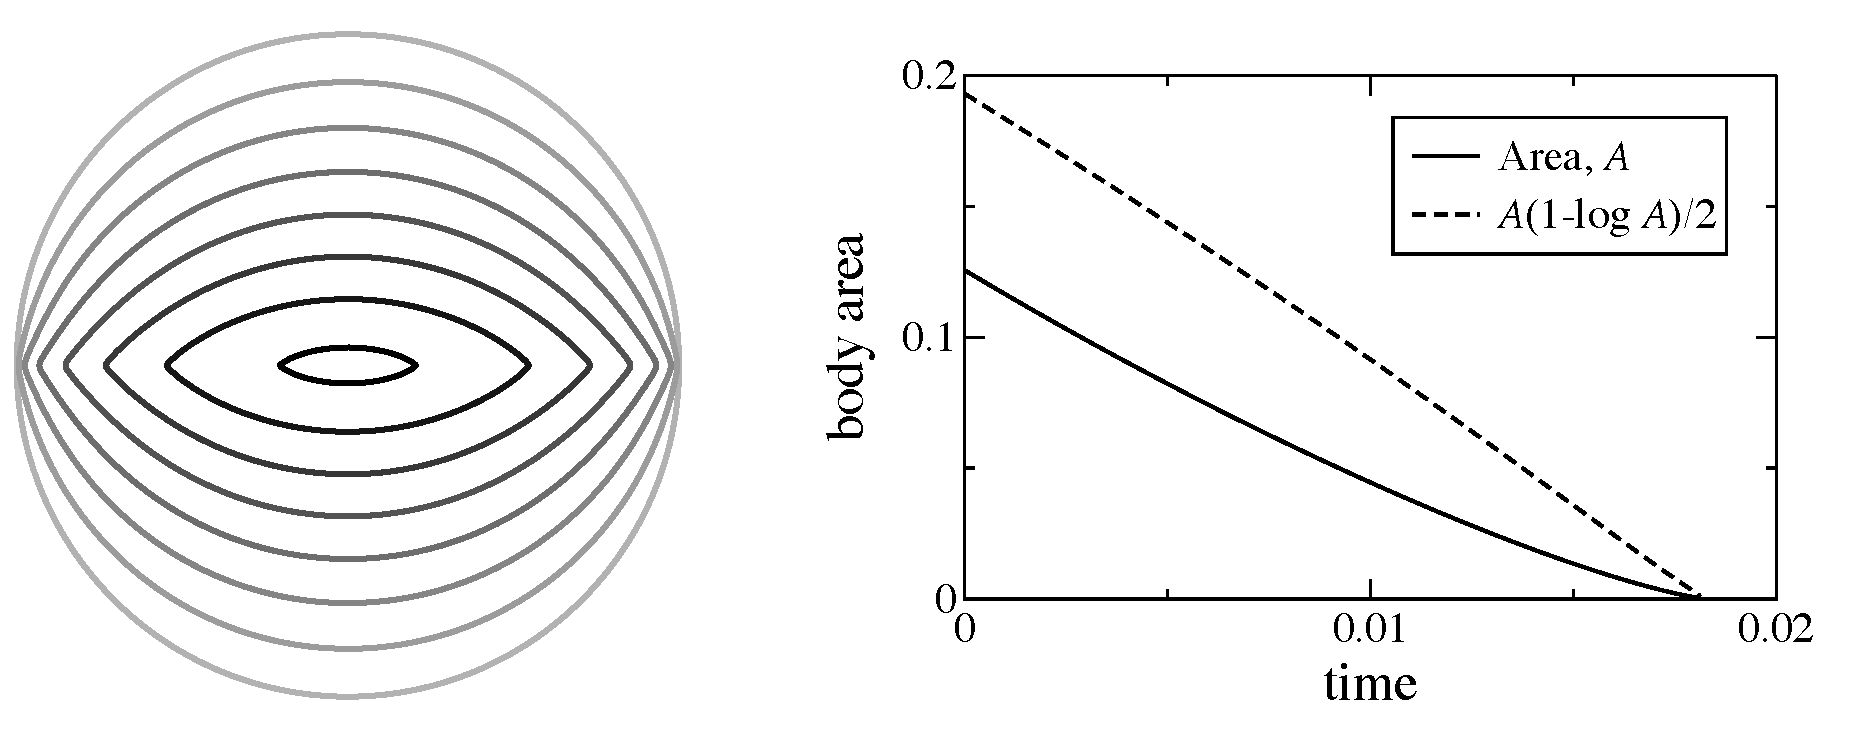
\includegraphics[width = 0.9 \textwidth]{./figs/fig3.pdf}
\caption{Shrinking body and area.}
\label{fig1}
\end{center}
\end{figure}
 %^^^^^^^^^^^^^^^^^^^^^^^^^^^^^^%

%^^^^^^^^^^^^^^^^^^^^^^^^^^^^^^%
\begin{figure}%[htbp]
\begin{center}
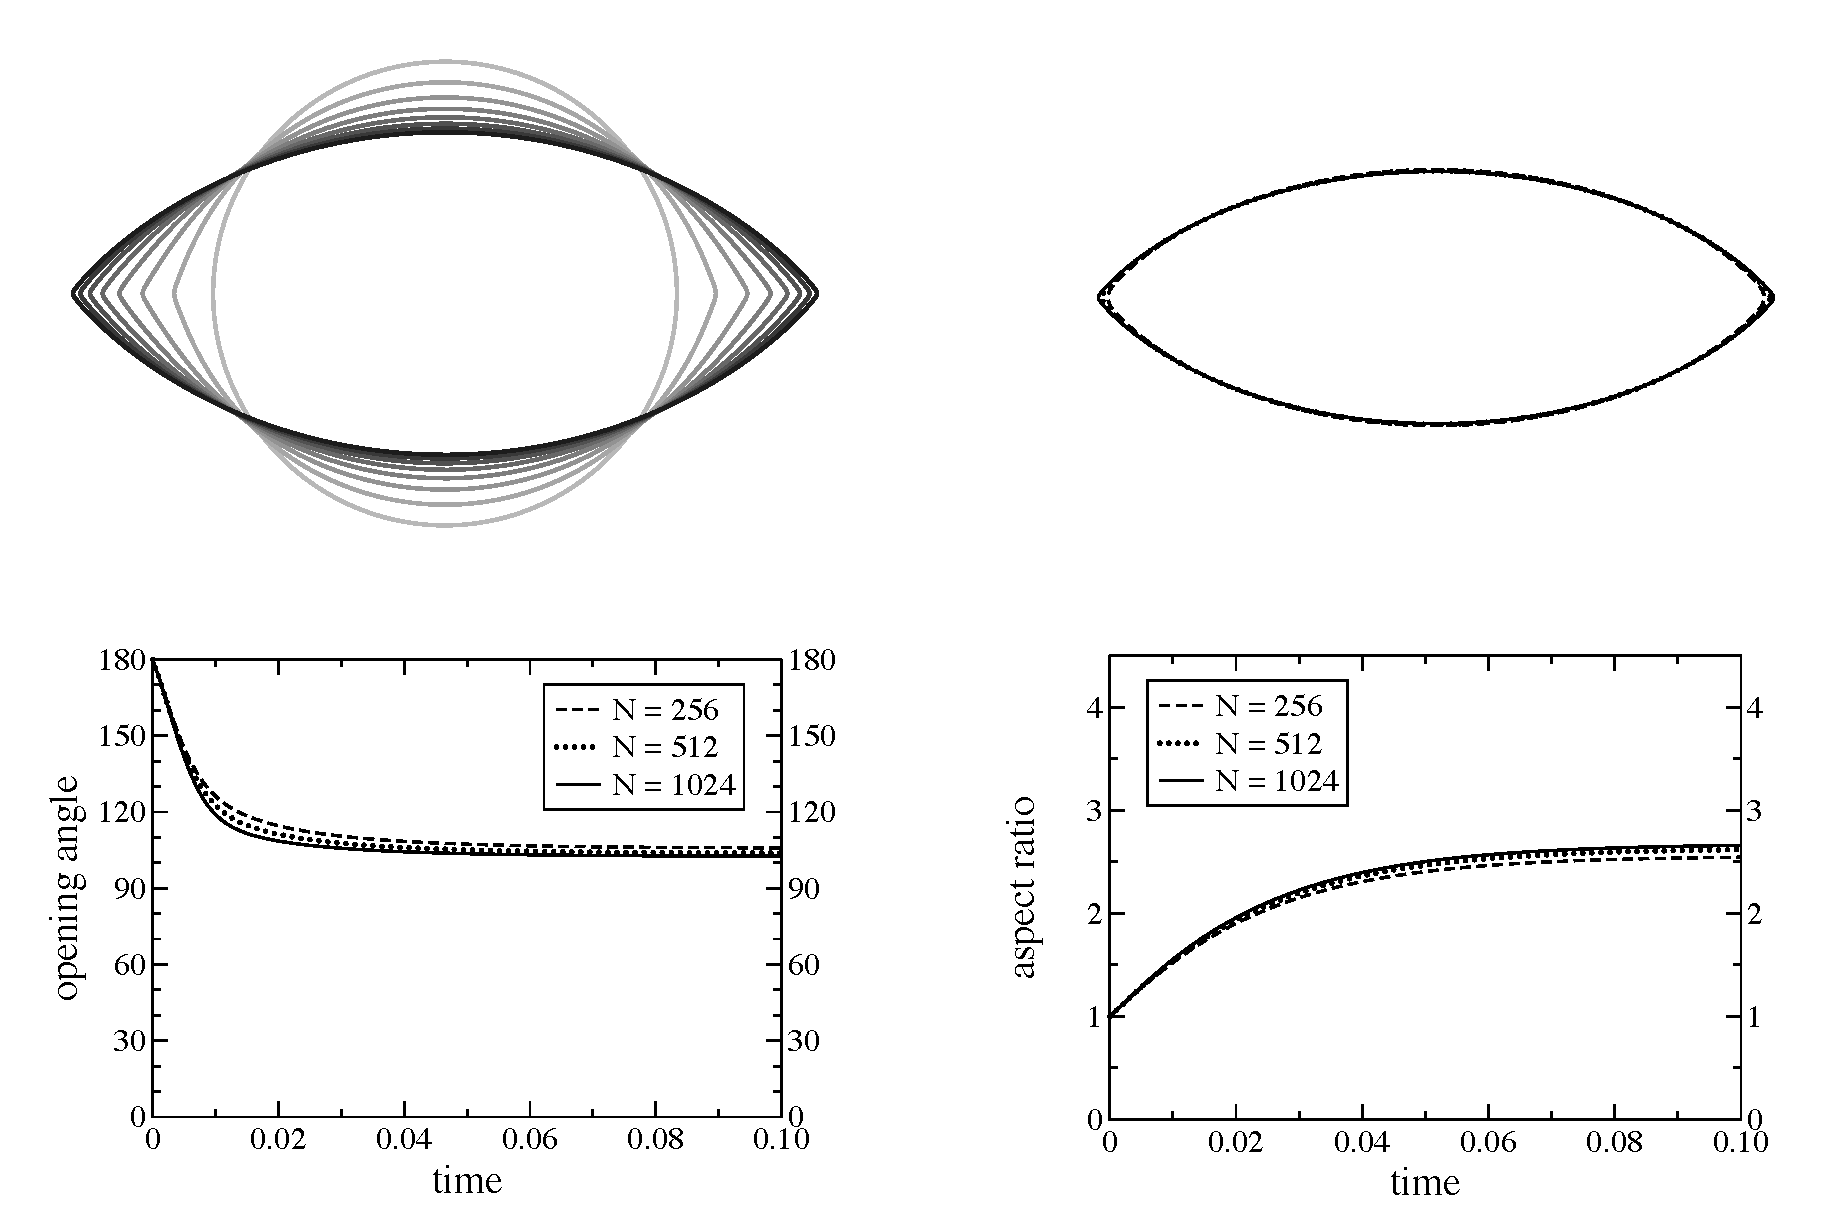
\includegraphics[width = 0.99 \textwidth]{./figs/fig4.pdf}
\caption{Final shape.}
\label{fig2}
\end{center}
\end{figure}
 %^^^^^^^^^^^^^^^^^^^^^^^^^^^^^^%

Runs to do
\begin{itemize}
  \item Single body
  \begin{itemize}
    \item Aspect ratio and opening angle
    \item Drag and resistivity
    \item Anisotropy
    \item Vorticity
  \end{itemize}
  \item $\bigO(5)$ bodies
  \begin{itemize}
    \item Drag and resistivity
    \item Anisotropy
    \item Long channels between flat faces
    \item Vorticity
  \end{itemize}
  \item $\bigO(50)$ bodies
  \begin{itemize}
    \item Drag and resistivity
    \item Anisotropy
    \item Vorticity
  \end{itemize}
\end{itemize}


%%%%%%%%%%%%%%%%%%%%%%%%%%%%%%%%%%%%%%%%%%%%%%%%%%%%%%%%%%%%%%%%%%%%%%%
\section{Conclusions\label{s:conclusions}}


%%%%%%%%%%%%%%%%%%%%%%%%%%%%%%%%%%%%%%%%%%%%%%%%%%%%%%%%%%%%%%%%%%%%%%%
\paragraph{\bf Acknowledgments} The authors would like to thank Manas Rachh
for supplying the FMM for the Stokes double-layer potential.


%%%%%%%%%%%%%%%%%%%%%%%%%%%%%%%%%%%%%%%%%%%%%%%%%%%%%%%%%%%%%%%%%%%%%%%
\begin{appendices}
\section{Error estimates for near-singular integration \label{A:AppendixA}} 
\end{appendices}


\bibliographystyle{plainnat} 
\bibliography{refs}
\biboptions{sort&compress}
\end{document}


